
\subsection{Building the Simulation Environment}

The simulation environment was implemented using the first-order macroscopic
Cell Transmission Model (CTM) as introduced by \cite{CTM}. The CTM discretises
a freeway section into homogeneous cells of equal length $\Delta x$ and evolves
traffic density forward in time according to:

\begin{equation}
    \rho_i(t+1)
    =
    \rho_i(t)
    +
    \frac{\Delta t}{\Delta x}
    \left[
    y_i(t) - y_{i+1}(t)
    \right]
\end{equation}

where $\rho_i(t)$ denotes the traffic density in cell $i$ at time $t$, $\Delta t$ the time interval between the steps $[t;t+1]$, and
$y_i(t)$ denotes the flow entering cell $i$ from its upstream neighbour.
The inter-cell flow is computed from separate sending and receiving functions:

\begin{equation}
    y_i(t) = \min\!\left\{ S_{i-1}(t),\; R_i(t) \right\}
\end{equation}

where:

\begin{equation}
    S_{i}(t) = \min\!\left\{ v_f\,\rho_{i}(t),\; Q_{i} \right\}
\end{equation}

\begin{equation}
    R_i(t) = \min\!\left\{ Q_i,\; w\!\left( \rho_i^{\mathrm{jam}} - \rho_i(t) \right) \right\}
\end{equation}

Here $v_f$ denotes the free-flow speed, $w$ the backward congestion-wave speed,
$Q_i$ the capacity of cell $i$, and $\rho_i^{\mathrm{jam}}$ its jam density.
The triangular fundamental diagram assumed throughout implies:

\begin{equation}
    w = \frac{Q_{\mathrm{lane}}}{\rho^{\mathrm{jam}}_{\mathrm{lane}} - \rho^{\mathrm{cr}}_{\mathrm{lane}}}
\end{equation}

An important restriction lies in the spatial and temporal discretisation, which must be selected to satisfy the
Courant--Friedrichs--Lewy stability condition (CFL) for explicit finite-difference
schemes \citep{CFL}, which in the CTM context requires that vehicles cannot
travel more than one cell during a single time step:

\begin{equation}
    \Delta x = v_f\,\Delta t
\end{equation}

\paragraph{Model parameters.}

The original study does not report the values of $\Delta x$ or $\Delta t$ used
in its simulations. To recover a consistent parameterisation, the model was
implemented in a modular fashion so that both quantities could be adjusted. A systematic exploration of feasible pairs satisfying the CFL
condition was conducted, and results were compared against the no-control
density contour reported by the authors. A cell length of
$\Delta x = 500\,\mathrm{m}$ with a corresponding time step of
$\Delta t = 15\,\mathrm{s}$ was found to reproduce the reported congestion
patterns satisfactorily.

The remaining fundamental diagram parameters were set as stated in the original
work: free-flow speed $v_f = 120\,\mathrm{km/h}$, critical density
$\rho^{\mathrm{cr}}_{\mathrm{lane}} = 20\,\mathrm{veh/(km{\cdot}lane)}$, and
jam density
$\rho^{\mathrm{jam}}_{\mathrm{lane}} = 100\,\mathrm{veh/(km{\cdot}lane)}$,
yielding a per-lane capacity of $Q_{\mathrm{lane}} = 2400\,\mathrm{veh/h}$.
Cell capacities and jam densities were scaled linearly with the local number of
lanes. The network layout follows Figure~3 of the original study: a
$6\,\mathrm{km}$ freeway section with a metered on-ramp at $2\,\mathrm{km}$
and a lane-drop from three to two lanes at $5.5\,\mathrm{km}$ downstream. The simulation horizon for each episode was set to $6000\,\mathrm{s}$.


\paragraph{Boundary conditions.}

The upstream boundary was implemented as a demand reservoir rather than as a
physical road cell. The inflow into the first road cell is therefore not
constrained by an upstream sending capacity, but by the available mainline
demand, any accumulated upstream queue $N_2$, and the receiving capacity of
the first cell:

\begin{equation}
    y_1(t) = \min\!\left\{ d_{\mathrm{main}}(t) + \frac{N_2(t)}{\Delta t},\;
    R_1(t) \right\}
\end{equation}

Any mainline flow that cannot enter the network accumulates in the upstream
queue:

\begin{equation}
    N_2(t+1) = \max\!\left\{ 0,\; N_2(t) + \bigl(d_{\mathrm{main}}(t) - y_1(t)\bigr)\,\Delta t \right\}
\end{equation}

At the downstream end of the network, free outflow was assumed. The outflow
from the final cell is determined solely by its sending function:

\begin{equation}
    y_{n}(t) = S_{n}(t)
\end{equation}

implying that congestion originating outside the simulated network cannot
propagate upstream into the modelled section.

\paragraph{On-ramp entry cell.}

The original study does not unambiguously specify into which cell the on-ramp
flow is injected. Based on Figure~3 of the original work, the ramp is located
at approximately $2\,\mathrm{km}$, which falls on the boundary between two
cells when $\Delta x = 500\,\mathrm{m}$. This ambiguity was resolved by
careful inspection of the spatio-temporal density contours reported in the
original study. Under the PI-ALINEA scenario, five characteristic congestion
waves are visible in the authors' results, propagating downstream and starting at
the $1500\,\mathrm{m}$ mark (see Figure~\ref{fig:pi_alinea_original_density_space_time_smoothed}). This
pattern is only consistent with ramp flow being injected into cell~4,
corresponding to the segment $1500$--$2000\,\mathrm{m}$, and was therefore
adopted throughout all experiments. The figure below (\ref{fig:Experimental_layout}) pictures the resulting experimental layout used.

\begin{figure}[H]
    \centering
    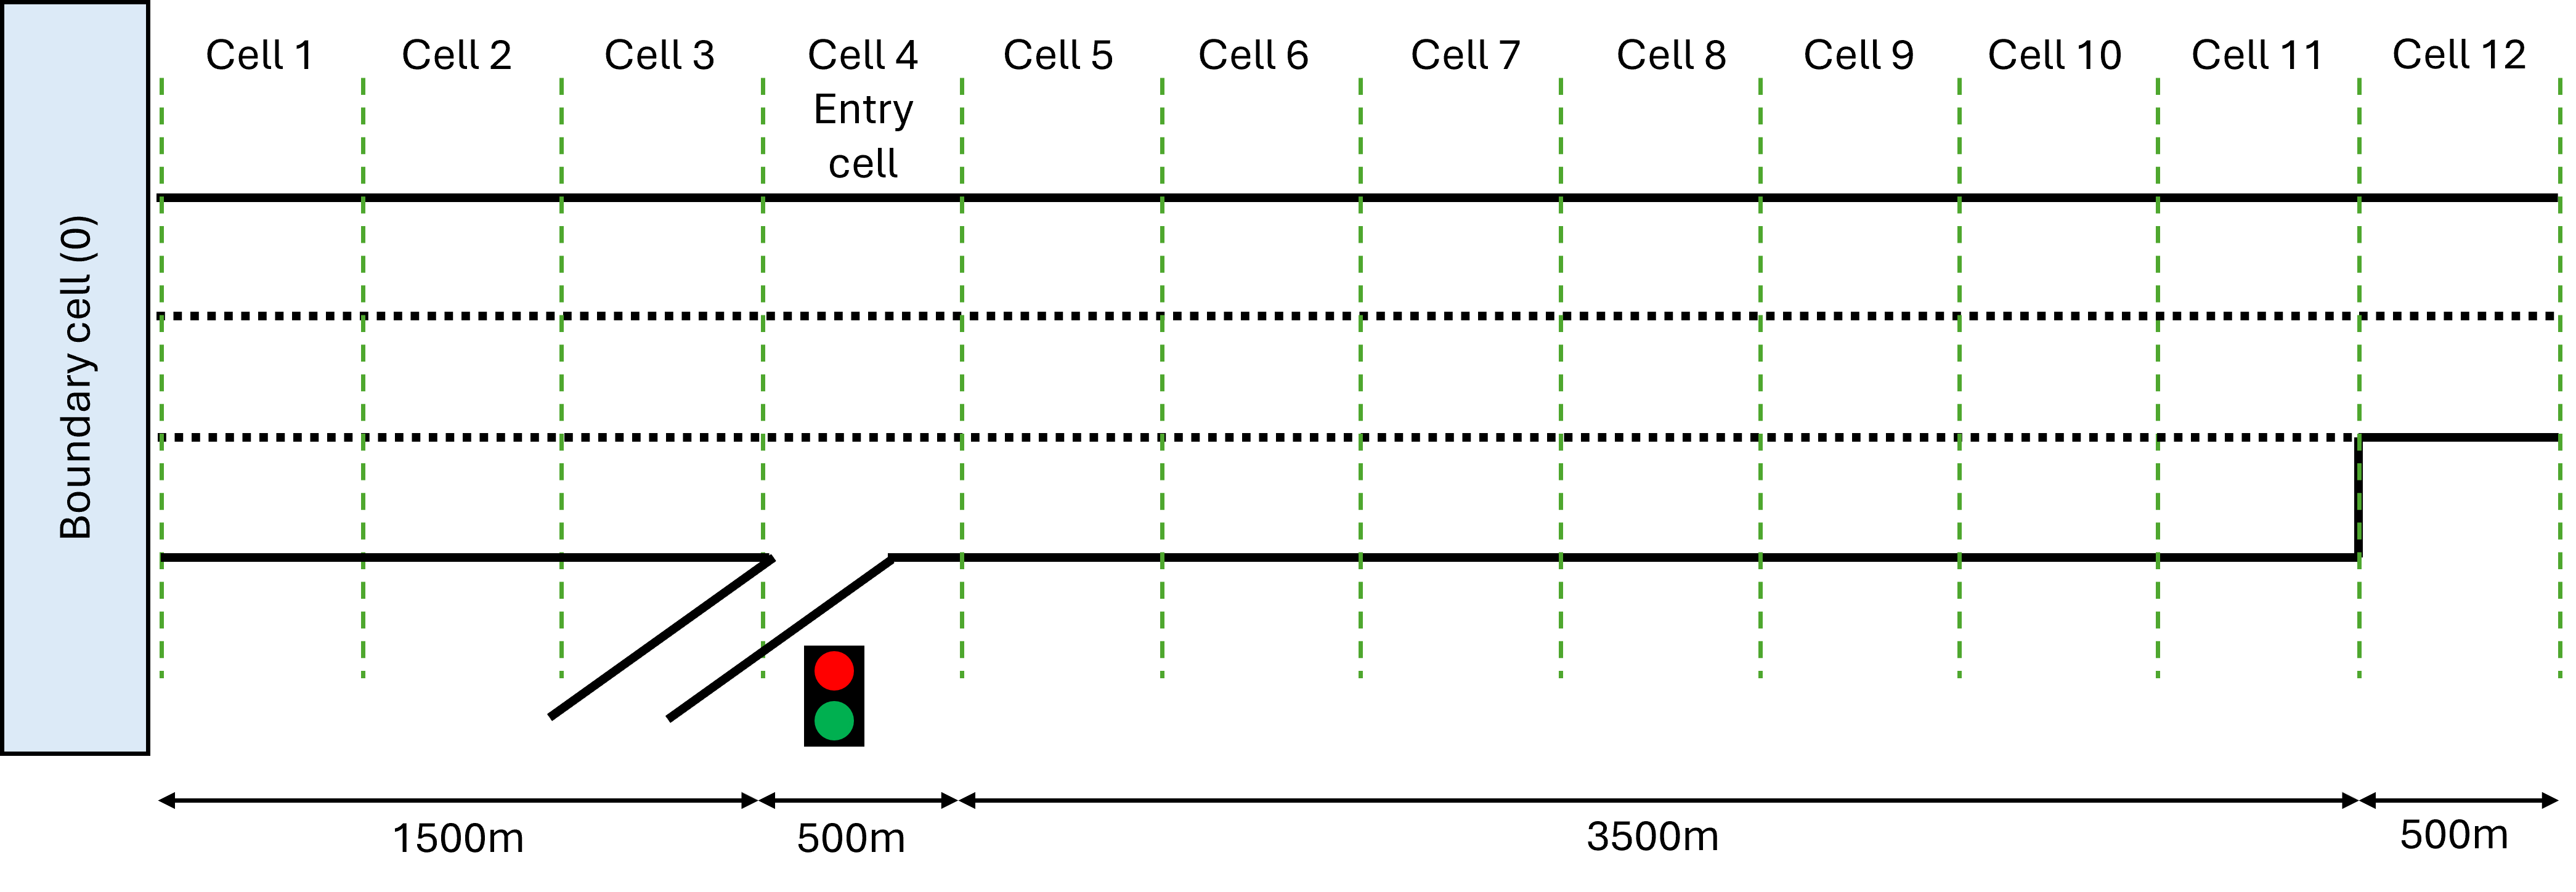
\includegraphics[width=1\linewidth]{figures/system_model.png}
    \caption{Layout of the freeway section used for the reproduction}
    \label{fig:Experimental_layout}
\end{figure}


\paragraph{Demand profile.}

The traffic demand profiles for the mainline and the on-ramp were not provided
numerically in the original study; only a figure of limited resolution was
available. The profiles were reconstructed through manual inspection of that
figure and iterative adjustment until the simulated no-control and PI-ALINEA control cell density diagram (see Figure~\ref{fig:comparison_no_control_control_cell_density} and \ref{fig:pi_alinea_original_control_cell_density}) and the PI-ALINEA ramp-metering rate (see Figure~\ref{fig:pi_alinea_original_metering_rate})
satisfactorily matched the published result.

The reconstructed profiles (see Figure \ref{fig:Demand_comparison}) follow a trapezoidal shape: a linear ramp-up of
$600\,\mathrm{s}$, a plateau of $1800\,\mathrm{s}$, and a symmetric ramp-down
of $600\,\mathrm{s}$, superimposed on constant baseline demands of
$1000\,\mathrm{veh/h}$ for the mainline and $500\,\mathrm{veh/h}$ for the
on-ramp. Peak demand increments of $3000\,\mathrm{veh/h}$ and
$720\,\mathrm{veh/h}$ were applied to the mainline and on-ramp respectively,
yielding maximum demands of $4000\,\mathrm{veh/h}$ and $1220\,\mathrm{veh/h}$.

\begin{figure}[ht]
    \centering
    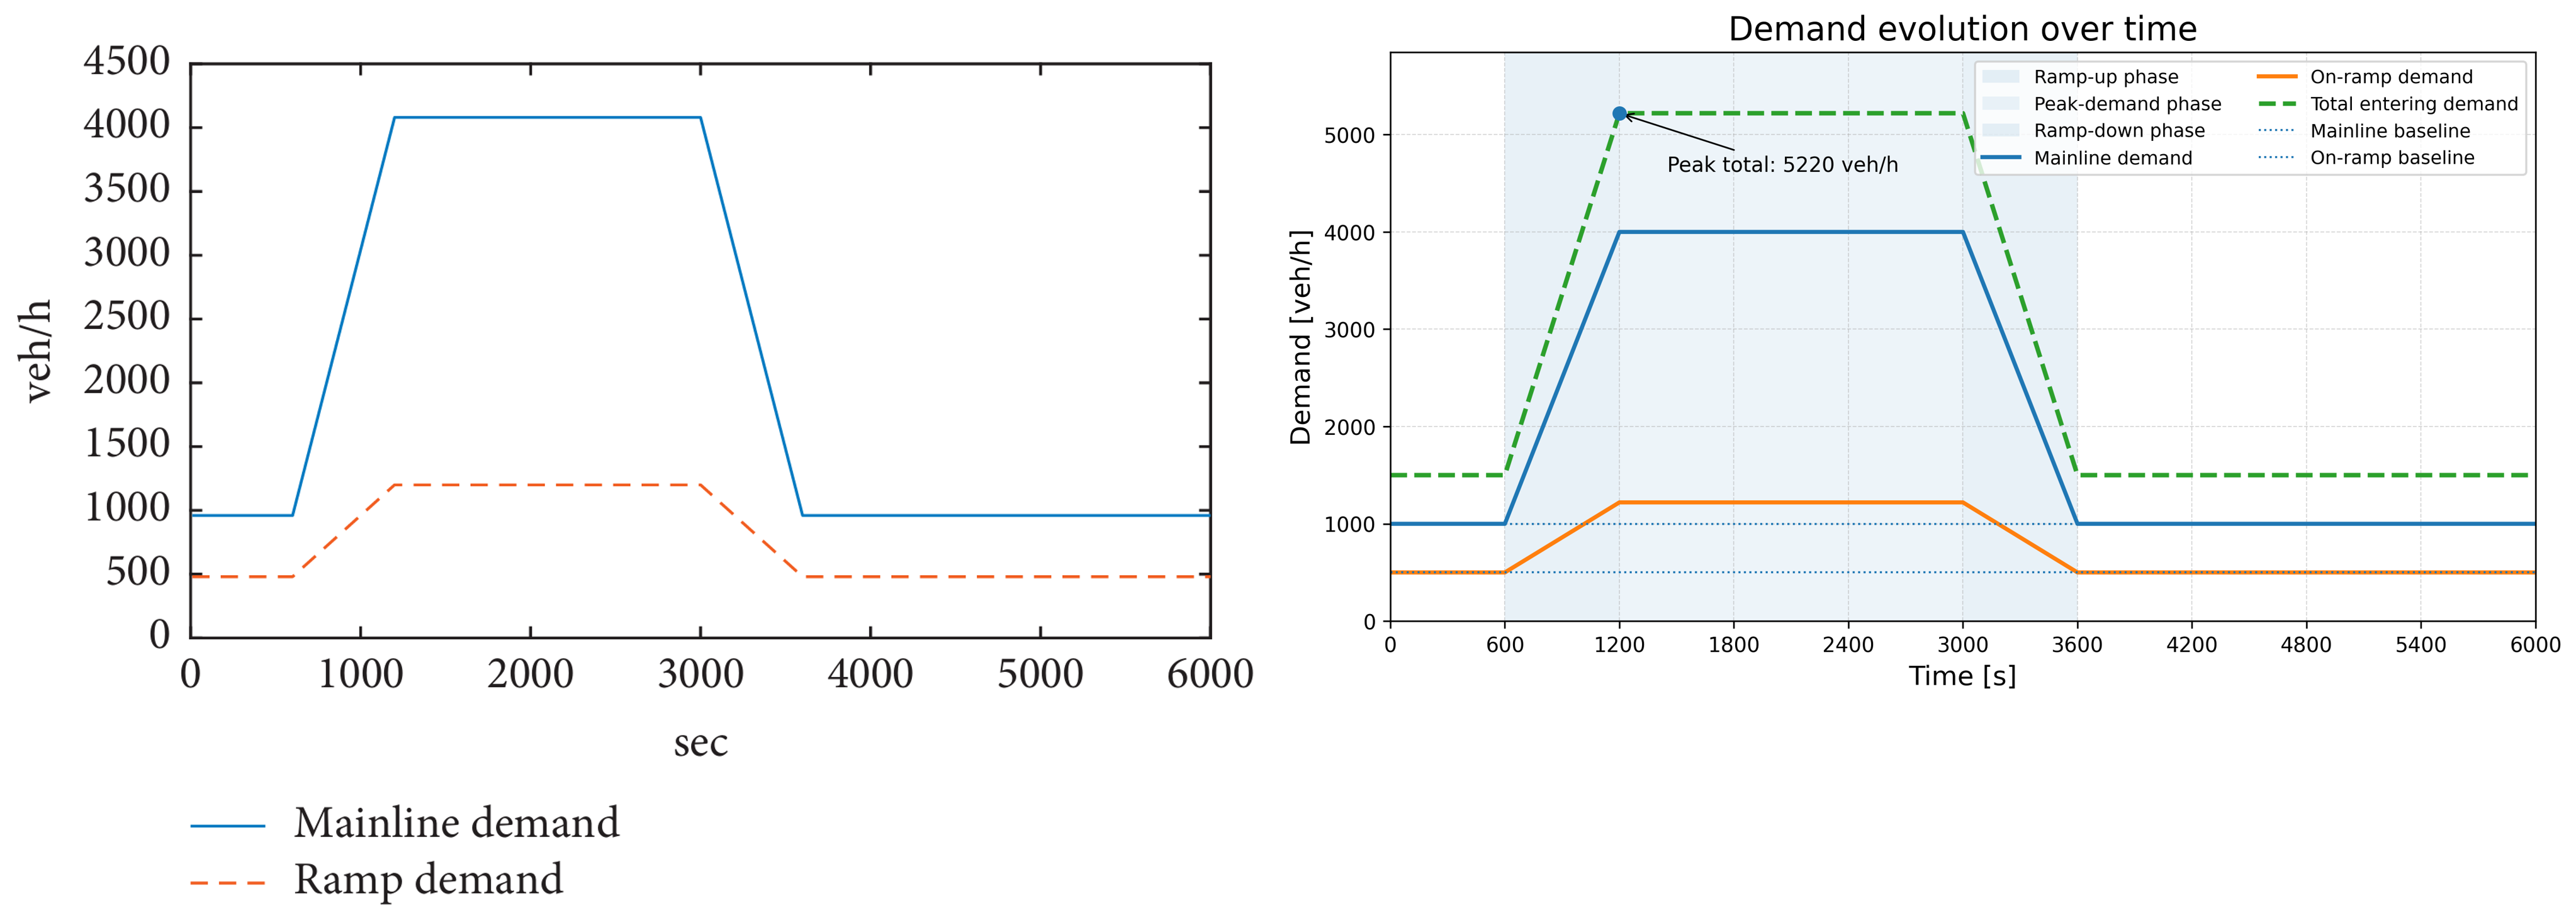
\includegraphics[width=1\linewidth]{figures/demand_comparison.png}
    \caption{Comparison of demand evolution in original study (left) and reproduction (right)}
    \label{fig:Demand_comparison}
\end{figure}

To facilitate exact reproduction, future studies are encouraged to report
demand profiles numerically alongside the simulation parameters $\Delta x$
and $\Delta t$, and to document explicitly the cell at which boundary flows
are injected.

\subsection{Implementation of the benchmark controllers}

\subsubsection{No-Control Scenario}

As a baseline for comparison, an uncontrolled scenario was implemented in which no ramp metering strategy was applied. In the absence of control actions, all on-ramp demand was released whenever sufficient downstream receiving capacity was available. If the combined mainline and ramp demand exceeded the receiving capacity of the downstream cell, the available capacity was distributed proportionally between the two streams.

The resulting traffic evolution serves as a reference case against which the effectiveness of the controllers can be evaluated.



\subsection{Benchmark Controllers: ALINEA and PI-ALINEA}

Two classical feedback-type ramp metering controllers were implemented as
benchmarks: ALINEA \citep{ALINEA} and its proportional--integral extension
PI-ALINEA \citep{PI-ALINEA}. PI-ALINEA is the sole benchmark considered in
the original study; ALINEA was additionally implemented in this replication
as a second more widely used baseline. Both controllers share the same
underlying control philosophy: regulate the on-ramp inflow so as to maintain
the traffic density at a designated control location close to a desired
setpoint, thereby preventing congestion formation at the downstream bottleneck
while maximising throughput.

\paragraph{ALINEA.}

ALINEA is a local proportional feedback controller that adjusts the metering
rate based solely on the deviation of the measured density from the desired
value. The control law reads:

\begin{equation}
    r(k) = r(k-1) + K_R\!\left[\hat{\rho} - \rho(k)\right]
\end{equation}

where $r(k)$ denotes the metering rate applied during control interval $k$,
$\rho(k)$ is the measured density at the control location, $\hat{\rho}$ is
the desired density, and $K_R$ is the integral gain. The controller increases
the metering rate when density falls below the set-point and reduces it when
density exceeds it, with no memory of past density errors beyond the previous
metering rate $r(k-1)$.

\paragraph{PI-ALINEA.}

PI-ALINEA extends ALINEA by adding a proportional term that reacts to the
rate of change of density, improving stability in the presence of time delays
such as those arising when the controlled bottleneck is located far downstream
of the metered ramp \citep{PI-ALINEA}. The control law is:

\begin{equation}
    r(k) = r(k-1) + K_R\!\left[\hat{\rho} - \rho(k)\right]
                  + K_P\!\left[\rho(k-1) - \rho(k)\right]
\end{equation}

where $K_P$ is the proportional gain and all other quantities are defined as
above. When $K_P = 0$ the expression reduces exactly to the ALINEA law,
making the two controllers structurally identical up to this single additional
term.

\paragraph{Implementation details.}

For both controllers, the control cell was set to cell~11, the last three-lane
cell immediately upstream of the lane-drop bottleneck
(see Figure~\ref{fig:Experimental_layout}), consistent with the formulation
of the original study. The desired density was set to
$\hat{\rho} = 13.33\,\mathrm{veh/(km{\cdot}lane)}$, corresponding to the
critical density scaled by the lane-drop ratio
$(\lambda_2/\lambda_1)\,\rho^{\mathrm{cr}}_{\mathrm{lane}} = (2/3)\times 20$,
as reported by the authors. Furthermore, in both cases, the metering rate was clipped to the admissible
range $[r_{\min}, r_{\max}] = [200, 1200]\,\mathrm{veh/h}$ at every control
step as stated in the original article to fit Full Traffic Cycle (FTC) restrictions according to \cite{Full_Traffic_Cycle}.

The original publication does not provide details of any controller
calibration procedure. Consulting the PI-ALINEA reference \citep{PI-ALINEA}
directly, the recommended gains for a distant bottleneck configuration are
$K_R = 4$ and $K_P = 100$, which were adopted without modification for
PI-ALINEA.


\subsubsection{Optimizing the Benchmark Controllers}

In addition to reproducing the benchmark controllers with the parameter values
used in the reference studies, a systematic grid search was conducted to assess
whether improved controller parameters could be identified. Two optimisation
criteria were considered: one evaluating mainline performance only, and one
additionally penalizing on-ramp queueing delay. The distinction reflects a
fundamental trade-off in ramp metering — aggressive metering improves mainline
flow but at the cost of accumulating ramp queues — and ensures that the
benchmark controllers are assessed from both a mainline and a system-wide
perspective.

\paragraph{Performance indicators.}

Both criteria are derived from vehicle-kilometres travelled (VKT) and
vehicle-hours travelled (VHT). For a given simulation run, VKT was computed as:

\begin{equation}
    \mathrm{VKT}
    =
    \sum_{k=1}^{N_t}
    \sum_{i=1}^{N}
    q_i(k)\,\Delta x\,\Delta t
\end{equation}

where $q_i(k)$ is the outflow of cell $i$ at time step $k$, $\Delta x$ is the
cell length, and $\Delta t$ is the simulation time step expressed in hours. The
mainline VHT was computed from the accumulated number of vehicles present in
the freeway cells:

\begin{equation}
    \mathrm{VHT}
    =
    \sum_{k=1}^{N_t}
    \sum_{i=1}^{N}
    \rho_i(k)\,\Delta x\,\Delta t
\end{equation}

The first optimisation criterion, targeting mainline performance only, is the
average network speed:

\begin{equation}
    \bar{v}
    =
    \frac{\mathrm{VKT}}{\mathrm{VHT}}
\end{equation}

which serves as a proxy for minimizing mainline total time spent (assuming there is no queue at the end of the simulation). Since this
criterion does not account for vehicles delayed in the on-ramp queue, a
queue-aware variant was introduced by augmenting VHT with the accumulated
ramp queue time:

\begin{equation}
    \mathrm{VHT}_{\mathrm{queue}}
    =
    \mathrm{VHT}
    +
    \sum_{k=1}^{N_t}
    N_1(k)\,\Delta t
\end{equation}

where $N_1(k)$ denotes the number of vehicles waiting in the on-ramp queue at
time step $k$. The queue-aware average speed

\begin{equation}
    \bar{v}_{\mathrm{queue}}
    =
    \frac{\mathrm{VKT}}{\mathrm{VHT}_{\mathrm{queue}}}
\end{equation}

constitutes the second optimisation criterion, providing a more system-oriented
measure of performance. When no residual ramp queue remains at the end of the
simulation, $\bar{v}_{\mathrm{queue}}$ closely approximates total system
performance. If a queue persists beyond the simulation horizon, however, the
true total time spent is still underestimated as the future delay of unserved
ramp vehicles is not captured.

\paragraph{Grid search.}

For ALINEA, the regulator gain was varied over the interval:
\begin{equation}
    K_R \in \{1, 2, \ldots, 110\}.
\end{equation}
For PI-ALINEA, both gains were varied over the same range:
\begin{equation}
    K_R \in \{1, 2, \ldots, 110\},
    \qquad
    K_P \in \{1, 2, \ldots, 110\}.
\end{equation}
Each parameter combination was evaluated over the full simulation horizon of
$6000\,\mathrm{s}$. The best-performing ALINEA and PI-ALINEA parameters were
identified separately under both optimisation criteria. These retuned
controllers were then compared with the original parameter choices and with
the RL-based controller in the subsequent evaluation.

\subsection{Building the RL-Agent}

The RL agent was implemented following Algorithm~1 of the original article and the architectural specifications of Section~3.4. The agent observes a four-dimensional continuous state vector at each time step, consisting of per-lane traffic densities sampled at three representative locations along the freeway stretch---$\rho_1$ at the upstream end of the stretch (cell~5, immediately downstream of the metered ramp), $\rho_2$ at the midpoint of the stretch (cell~8), and $\rho_3$ at the control target cell (cell~11, immediately upstream of the lane-drop)---alongside the estimated ramp demand $D_{\mathrm{ramp}}$ computed from the current on-ramp queue length and the previous time step's actual ramp inflow, following equation~1 of the original work. For a graphic representation of the cells locations, see Figure \ref{fig:Experimental_layout}. Note that the exact cell numbers are not explicitly stated in the source article, but could be easily identified with the help of the original figure 1 once the cell dimensions were identified. 

Prior to being fed into the neural network, the continuous state vector is encoded into a 140-dimensional binary feature vector using a tile coding scheme \citep{EPSILON_GREEDY}; each of the three density variables is mapped to one of 40 equal-width bins covering the range $[0,\rho_{\mathrm{jam,lane}}] = [0,100]\,\mathrm{veh/km/lane}$, and $D_{\mathrm{ramp}}$ is mapped to one of 20 bins, the first 19 covering $[0,a_{\max}] = [0,1200]\,\mathrm{veh/h}$ uniformly and the last bin capturing any value above $a_{\max}$, the highest possible action. This follows the encoding described in the study. However, as the on-ramp demand never falls bellow 500 $\mathrm{veh/h}$ during training, 37\%  of the encoding space of the ramp demand ends up never getting used during training. A simple, more optimised alternative would be to cover the interval $[0;500]\,\mathrm{veh/h}$ with 1 bin, $ [500,1200]\,\mathrm{veh/h}$ with 18 bins, and 1 final bin for values above $a_{\max}$.

The approximate value function is a fully connected artificial neural network (ANN) with a 140-dimensional input layer, a single hidden layer of 420 neurons, and an output layer of 11 neurons corresponding to the 11 discrete admissible metering rates $\{200,300,\ldots,1200\}\,\mathrm{veh/h}$, to again accommodate FTC recommendations \citep{Full_Traffic_Cycle}. The hidden layer uses a sigmoid activation function, as explicitly specified in the original paper. The output layer is linear, so Q-values can take any real value, positive or negative, unbounded.

A critical implementation challenge arose from the combination of sigmoid
activation, online stochastic gradient descent (SDG, i.e., incremental back-propagation), bootstrapped Q-learning targets,
and the unbounded linear output layer for the Q-values. Sigmoid activations can
saturate for large input magnitudes, causing their derivatives to become very
small and thereby degrading gradient propagation
\citep{XAVIER_INITIALIZATION}. Since the original article
only states that the ANN parameters were initialised with small random values,
without specifying a reproducible initialisation scheme, Xavier--Glorot uniform
initialisation was used for both linear layers \citep{XAVIER_INITIALIZATION}.
In addition, gradient clipping with a maximum norm of 1.0 was applied at each
update step to limit occasional exploding gradients
\citep{GRADIENT_CLIPPING}.

The network is trained using online SGD---one gradient step per time step---with a two-phase learning rate schedule: $\alpha = 0.05$ for the first 100,000 episodes and $\alpha = 0.01$ thereafter, following the paper's specification. The discount factor is $\gamma = 0.95$, as stated in the paper. The reward signal at each step is:
\begin{equation}
    r = k \cdot |\rho_3 - \rho_{\mathrm{des}}|
\label{eq:reward_function}    
\end{equation} where $k$ is a user-defined negative scaling constant. The paper does not specify the value of $k$; in this implementation, $k = -1.0$ was used. Action selection follows an $\epsilon$-greedy policy with $\epsilon$ decaying over the course of training. At each time step, the admissible action set is constrained from above by the estimated ramp demand $D_{\mathrm{ramp}}$, preventing the agent from selecting a metering rate that exceeds the available ramp flow.

Training was conducted for 700,000 episodes, each corresponding to one full simulation of the $6000\,\mathrm{s}$ demand scenario using the Cell Transmission Model as the environment. The original article reports that
learning converged after approximately 0.7 million episodes, but does not
specify the precise convergence criterion or the decay schedule used for the
\(\epsilon\)-greedy exploration policy. Therefore, training was run for the
reported 700,000 episodes in all experiments.

Since the exploration decay was not specified, an exponential decay factor of
\(0.99999\) was adopted for \(\epsilon\), starting from
\(\epsilon_0 = 1.0\). With this setting, the exploration rate reaches
approximately \(5\%\) after about 300,000 episodes. Two exploration variants
were tested: one in which \(\epsilon\) was allowed to continue decaying without
a lower bound, and one in which a minimum exploration rate of
\(\epsilon_{\min}=0.05\) was retained. The latter follows common reinforcement
learning practice, where a non-zero exploration floor is often used to avoid
premature convergence to a deterministic policy \citep{EPSILON_GREEDY_CAP}.

 Network checkpoints were saved every 10,000 episodes to allow recovery from interruptions and to enable retrospective evaluation of policy quality at different stages of training. Software and computational environment specifications can be seen in the appendix \ref{sec:a-Software}.




%\clearpage